%
%  ARTIE paper
% 
%  Compling:
%  1)  pdflatex main.tex
%  2)  bibtex main
%  3)  pdflatex main.tex
%  4)  pdflatex main.tex
%
\documentclass[%
 reprint,
superscriptaddress,
 preprintnumbers,
 nofootinbib,
 nobibnotes,
 bibnotes,
 amsmath,amssymb,
 aps,
 prl, 
 floatfix,
]{revtex4-1}

\usepackage{graphicx}% Include figure files
\usepackage{dcolumn}% Align table columns on decimal point
\usepackage{bm}% bold math
\usepackage{comment}% Commented text stays on .tex document but not on pdf
\usepackage{xcolor}
\usepackage{natbib}
\usepackage[nowatermark]{fixmetodonotes}
\usepackage{isotope}
\usepackage{verbatim}
\usepackage{siunitx}
% Use an ordinary space between a number and its associated unit
\sisetup{number-unit-product=\ }
% Don't use a space between a number and the percent sign
\DeclareSIUnit[number-unit-product = ]\percent{\char`\%}

\usepackage{hyperref}% add hypertext capabilities
\usepackage[mathlines]{lineno}% Enable numbering of text and display math
%\linenumbers\relax % Commence numbering lines

%\usepackage[showframe,%Uncomment any one of the following lines to test 
%%scale=0.7, marginratio={1:1, 2:3}, ignoreall,% default settings
%%text={7in,10in},centering,
%%margin=1.5in,
%%total={6.5in,8.75in}, top=1.2in, left=0.9in, includefoot,
%%height=10in,a5paper,hmargin={3cm,0.8in},
%]{geometry}

\newcommand{\eV}{\mathrm{e\kern -0.1em V}}
\newcommand{\MeV}{\mathrm{Me\kern -0.1em V}}
\newcommand{\keV}{\mathrm{ke\kern -0.1em V}}

\begin{document}

%\preprint{APS/123-QED}

\title{Measurement of the total neutron cross section on argon in the energy range $30-70 \keV$} % Force line breaks with \\

\author{S. Andringa}
\affiliation{Laborat{\'o}rio de Instrumenta{}{\c c}{\~a}o e F{\'i}sica Experimental de Part{\'i}culas (LIP), Av. Prof. Gama Pinto, 2, 1649-003, Lisboa, Portugal}

\author{Y.Bezawada}
\affiliation{University of California at Davis, Department of Physics, Davis, CA 95616, U.S.A.}

\author{T. Erjavec}
\affiliation{University of California at Davis, Department of Physics, Davis, CA 95616, U.S.A.}

\author{J. He}
\affiliation{University of California at Davis, Department of Physics, Davis, CA 95616, U.S.A.}

\author{J. Huang}
\affiliation{University of California at Davis, Department of Physics, Davis, CA 95616, U.S.A.}

\author{P. Koehler}
\affiliation{Los Alamos National Laboratory, LANSCE, Los Alamos, NM 87545, U.S.A.}

\author{M. Mocko}
\affiliation{Los Alamos National Laboratory, LANSCE, Los Alamos, NM 87545, U.S.A.}

\author{M. Mulhearn}
\affiliation{University of California at Davis, Department of Physics, Davis, CA 95616, U.S.A.}

\author{L. Pagani}
%\email{lpagani@ucdavis.edu}
\affiliation{University of California at Davis, Department of Physics, Davis, CA 95616, U.S.A.}

\author{E. Pantic}
\affiliation{University of California at Davis, Department of Physics, Davis, CA 95616, U.S.A.}

\author{L. Pickard}
\affiliation{University of California at Davis, Department of Physics, Davis, CA 95616, U.S.A.}

\author{R. Svoboda}
\affiliation{University of California at Davis, Department of Physics, Davis, CA 95616, U.S.A.}

\author{J. Ullmann}
\affiliation{Los Alamos National Laboratory, LANSCE, Los Alamos, NM 87545, U.S.A.}

\author{J. Wang}
\affiliation{University of California at Davis, Department of Physics, Davis, CA 95616, U.S.A.}
\affiliation{South Dakota School of Mines and Technology, Physics Department, Rapid City, SD 57701 USA}

\collaboration{ARTIE Collaboration}%\noaffiliation

\date{\today}
             
\begin{abstract}

Argon


  is a widely used detector medium 

A wide range of experiments which are 
  investigating dark matter and neutrinos.


neutrino and dark matter experiments has made the precise knowledge of
the cross section for neutron interactions on argon an important
design and operational parameter. Nevertheless, there has been a
lingering discrepancy between the total cross-section in the 30-70 keV
region given in the Evaluated Nuclear Data File (ENDF) and the single
measurement done in the 1990's by an experiment optimized for higher
energy. This discrepancy is significant in that the former predicts a
large negative resonance in the region while the measurement did not
report such a feature, giving rise to significant uncertainty in the
penetration depth of neutrons through liquid argon. This paper
presents results from the Argon Resonant Transport Interaction
Experiment (ARTIE) at the Los Alamos Neutron Science Center (LANSCE),
the first dedicated experiment optimized for this energy region. The
ARTIE measurement of the total cross-section as a function of energy
confirms the existence of a negative resonance in this region, but not
quite as deep as the ENDF prediction.

\end{abstract}

\pacs{28.20.Cz}% PACS, the Physics and Astronomy 

                             % Classification Scheme.
%\keywords{Suggested keywords}%Use showkeys class option if keyword
                              %display desired
\maketitle

%\tableofcontents

\section{\label{sec:intro}Introduction}

Argon is used in a wide range of particle physics experiments
investigating neutrinos~\cite{Antonello:2013ypa, Acciarri:2016smi,
  Abi:2017aow, Acciarri:2016ooe}, dark matter~\cite{DEAP:2019,
  Aalseth:2017fik}, and neutrinoless double beta
decay~\cite{Ackermann:2012xja, Abgrall:2017syy}.  Achieving many of
the scientific objectives sought by these experiments relies on
understanding the transport of neutrons through liquid argon at a
level of precision which has only recently emerged as a critical
experimental requirement.  A recent measurement of the neutron capture
cross-section~\cite{Fischer2019b, Fischer2019a} settled a roughly
$50\%$ discrepancy between previous measurements in favor of the ENDF
cross-sections\cite{ENDF} for neutron kinetic energy below $1~\eV$.

The neutron-argon total cross-section as predicted by ENDF features an
anti-resonance feature at $57~\keV$ which increases the neutron
interaction length in liquid argon, for a natural abundance of
isotopes, to $42~\rm m$.  At this energy scale, neutrons only lose a
fraction of their kinetic energy during each elastic collision with a
relatively massive argon nuclei, and so even neutrons with kinetic
energy well above $57~\rm keV$ eventually reach the anti-resonance
feature and the resulting long interation length.  The results of the
most recent previous measurement~\cite{Winters:1991} were inconsistent
with ENDF in the region of the anti-resonance feature, with an
inferred interaction length of $6~\rm m$.  The discrepancy makes it
impossible to reliably predict the effectiveness of fiducial volume
cuts in liquid argon to suppress neutrons from outside of the
detector.  In large TPCs like DUNE, neutrons from neutrino
interactions will escape the detector volume at an unknown rate, which
might impact the energy resolution.  The design of calibration systems
which use externally produced neutrons relies critically on the
precise depth of the anti-resonance feature.  This paper describes the
Argon Resonance Transport Interaction Experiment (ARTIE) which was
designed for the sole purpose of resolving the discrepancy.

ARTIE features an experimental determination of the transmission
coefficient $T$, defined as the fraction of neutrons which pass
through a custom liquid argon target without scattering.  For a
target of length $d$ with atomic number density $n_{\rm trg}$, the
cross-section is given by:
\begin{equation}
  \sigma = -\frac{1}{n_{\rm trg} \, d} \, \ln \, T.
\label{eq:sigma}
\end{equation}
The target thickness $n_{\rm trg} d$ is a critical experimental
parameter, and the ARTIE target was designed to have a thickness
approximately twenty times larger than Ref.~\cite{Winters:1991}, which
casts the cross section discrepancy as competing predictions for
transmission coefficient for the ARTIE target of either
{\color{red} $X$ or $Y$}.
The ARTIE target is well suited to the anti-resonance region, but
quickly becomes opaque to neutrons at higher cross-section.  Our
energy region of interest is defined as $30$ to $70~\rm keV$.

\section{\label{sec:setup}Experimental Methods}

The ARTIE target is a column of liquid argon with a length of $168~\rm
cm$ and a diameter of $25~\rm mm$, held at atmospheric pressure, and
contained in a vessel constructed from commercial components.  For
transparency to neutrons, the ends of the target were fashioned from
kapton foil compressed against a teflon seal in a standard commercial
flange.  The kapton foil was flushed with gaseous dry nitrogen
continuously during operation to minimize ice formation.

The target was inserted into Flight Path\,13 (FP13) of the Lujan
Neutron Scattering Center~\cite{LANSCEBeam:1990} at a distance $31~\rm
m$ from the upper-tier liquid hydrogen moderator of the
accelerator-driven pulsed neutron source. The Mark III
Target-Moderator-Reflector-Shield (TMRS)~\cite{moderator} is driven by
an $800~\MeV$ proton linac that produces a $250~\rm ns$ triangular
pulse at a repetition rate of $20~\rm Hz$ and a typical beam current
of $80~\rm \mu A$. Neutrons are produced via spallation reactions
inside a tungsten target with a $1/E$ energy spectrum.  During data
taking, the proton beam current as measured by a current transformer
(CT) sensor is recorded once per minute.

The flight path includes a neutron detector, located approximately
$30~\rm m$ downstream of the target, consisting of a $9~\rm cm$
diameter by $1~\rm mm$ thick $^6$Li-glass scintillator, viewed edge-on
by two Burle 8854 five-inch photomultiplier tubes (PMTs).  We define a
neutron event as a pulse above a fixed threshold in ether PMT.  The
data acquisition system records a timestamp and integrated charge for
several time intervals for each neutron event.  {\color{red} Describe
  relationship between timestamp and measured TOF.}

Three-inch thick cylindrical blocks of brass with $6~\rm mm$ holes in
the center were used to collimate the beam near the target.  Two such
collimators were located upstream of the target, and two downstream.
When aligned, the collimators constrain the beam to the interior of
the $25~\rm mm$ diameter target, and produce a beam spot with an
$8~\rm cm$ diameter at the $9~\rm cm$ diameter neutron detector.  The
final alignment of the collimators was based on beam profile images
obtained from storage-phosphor image plates placed at the $^{6}$Li
detector.  Following several iterations, a symmetric image was
obtained and the neutron event rate reached a plateau.

For a cost effective design, the ARTIE target uses rigid foam
insulation designed for cryogenic applications.  Near each ends of the
target vessel, an opening upward feeds into a commerical plastic
dewar.  As argon boils in the detector, gaseous argon vents through
the openings and is replaced by liquid argon from the dewars.  During
normal operation, the dewars were refilled remotely about once per
hour to ensure that the target remained full.

The ARTIE experiment collected data during a two week period beginning
in October 2019, with most of the data taken in either of two target
configurations.  During target-in runs, the target vessel was filled
with liquid argon (LAr).  During target-out runs, the target vessel
was continuously flushed with gaseous argon (GAr).  The transmission
coefficient is experimentally determined as:
\begin{equation}
T = \frac{N_{\rm in} - B_{\rm in}}{N_{\rm out} - B_{\rm out}}\cdot\frac{Q_{\rm out}}{Q_{\rm in}}
\label{eq:T}
\end{equation}
where $N_{\rm in}$ and $N_{\rm out}$ are the number of neutrons
observed in the neutron detector during target-in and target-out runs,
$Q_{\rm in}$ and $Q_{\rm out}$ are the time integrated beam currents
as determined from the CT sensor, and $B_{\rm in}$ and $B_{\rm out}$
are experimentally determined background rates.  The transmission
coefficient $T$ is calculated in bins of TOF, which are calibrated to bins in neutron kinetic energy.

\begin{table}[htb]
\begin{tabular}{|c|c|c|c|c|c|c|}
\hline
target & live     & after    &   & neutron & selected & total \\
fill   & time (h) & cuts (h) & Q & events  & neutrons & ROI \\
\hline
Gas     & 2.7056e+08 & & & & &  \\
Liquid  & 1.1323e+08 & & & & &  \\
\hline
\end{tabular}
\caption{{\color{red} This table to be updated by Jingbo...}}
\label{tab:cutflow}
\end{table}

The neutron counts used in Eq.~\ref{eq:T} are counts of neutron events which
survive time-dependent run quality cuts and neutron selection
cuts, as summarized in Table~\ref{tab:cutflow}.  To minimize the
impact of non-linearity between the CT sensor and the neutron beam
intensity, the analysis only includes the $95\%$ of collected data
taken while the beam current was near the maximum value.  Periods of
instability in the data acquisition system, which were occassionally
observed as a precipitous drop in neutron event rate while the beam
current was constant, were also removed from the analysis.  A dramatic
decrease in the beam-intensity normalized neutron event rate was
observed each time the dewars were filled with liquid argon.  The rate
returned to a plateau value during the 15-20 minute period that
followed each filling.  While filling the target, significant amounts
of liquid argon vapor and gas would spill onto the brass collimators
downstream of the target.  We suspect that this caused the collimators
to move out of alignment and then realign as the collimators returned
to room temperature.  We removed the $12\%$ of liquid argon data from
the periods during and following filling when the beam-current
normalized neutron rate was less than 95\% of the plateau value.
Neutron selection cuts require both PMTs to register pulses within a 
$100~\rm ns$ coincidence window, and {\color{red} to pass a cut which removes retriggered events.}

\section{\label{sec:energy}Background Determination}

Determination of the argon transmission coefficient in
Equation~\ref{eq:T} relies on subtracting background events, both
those arising from non-neutron sources, such as radiogenic background,
and from neutrons (or secondary particles) with a measured TOF
inconsistent with the neutron kinetic energy.  Data collected while
the beam was off indicates that beam independent background is
negligible in the ROI.  Data collected with the beam on but a
mechanical iron shutter closed before the flight path showed that
background from the acellerator complex, such as skyshine or
scattering from other experiments, is likewise neglible, as the
resulting events arrive quite late, well outside of our ROI.  The
background from slow neutrons, which could alias as faster neutrons
from a later pulse, is effectively eliminated by the addition of a
0.16 cm thick cadmium filter.  The cadmium filter supresses neutrons
with kinetic energy below $0.5~\rm eV$, and the remaining neutrons
arrive reliably within the $50~\rm ms$ between pulses.

The tight timing requirement significantly reduces background from
random noise and PMT after pulsing.

Our $9~\rm cm$ neutron detector is located about $30~\rm m$ from the
target, presenting a tiny solid angle for neutrons that might reach
the detector through secondary scattering.  Our analysis indicates
that the major background contribution is consistent with neutrons
which reach the near detector and undergo multiple scattering near the
detector.  The correlation between time-of-flight and neutron energy
is lost for these events, and the resulting background is flat in TOF
across our region of interest.  To estimate the background $B$
present in neutron counts $N$ we run under identifical conditions
apart from the insertion of a $2.5~\rm cm$ thick aluminum filter into
the beam-line.  From the resulting neutron counts $N_{Al}$ scaled
to the same exposure as $N$ we calculate the background as:
\begin{equation}
  B = \frac{N_{\rm Al} - T_{\rm Al} \cdot N}{1-T_{\rm Al}}
\label{eq:B}
\end{equation}
where $T_{\rm Al}$ is the known transmission coefficient of the
aluminum filter, smeared by energy resolution.  This technique \cite{Brown:2017accapp} uses the
narrow resonances near our region of interest in the neutron-aluminum
cross-section to provide a peek at the background.  The amount by
which count $N_{\rm Al}(E)$ in a narrow resonance exceeds the
projected count from the known aluminum transmission $T \cdot N$
indicates the amount of background.

\begin{figure}[htbp]\centering
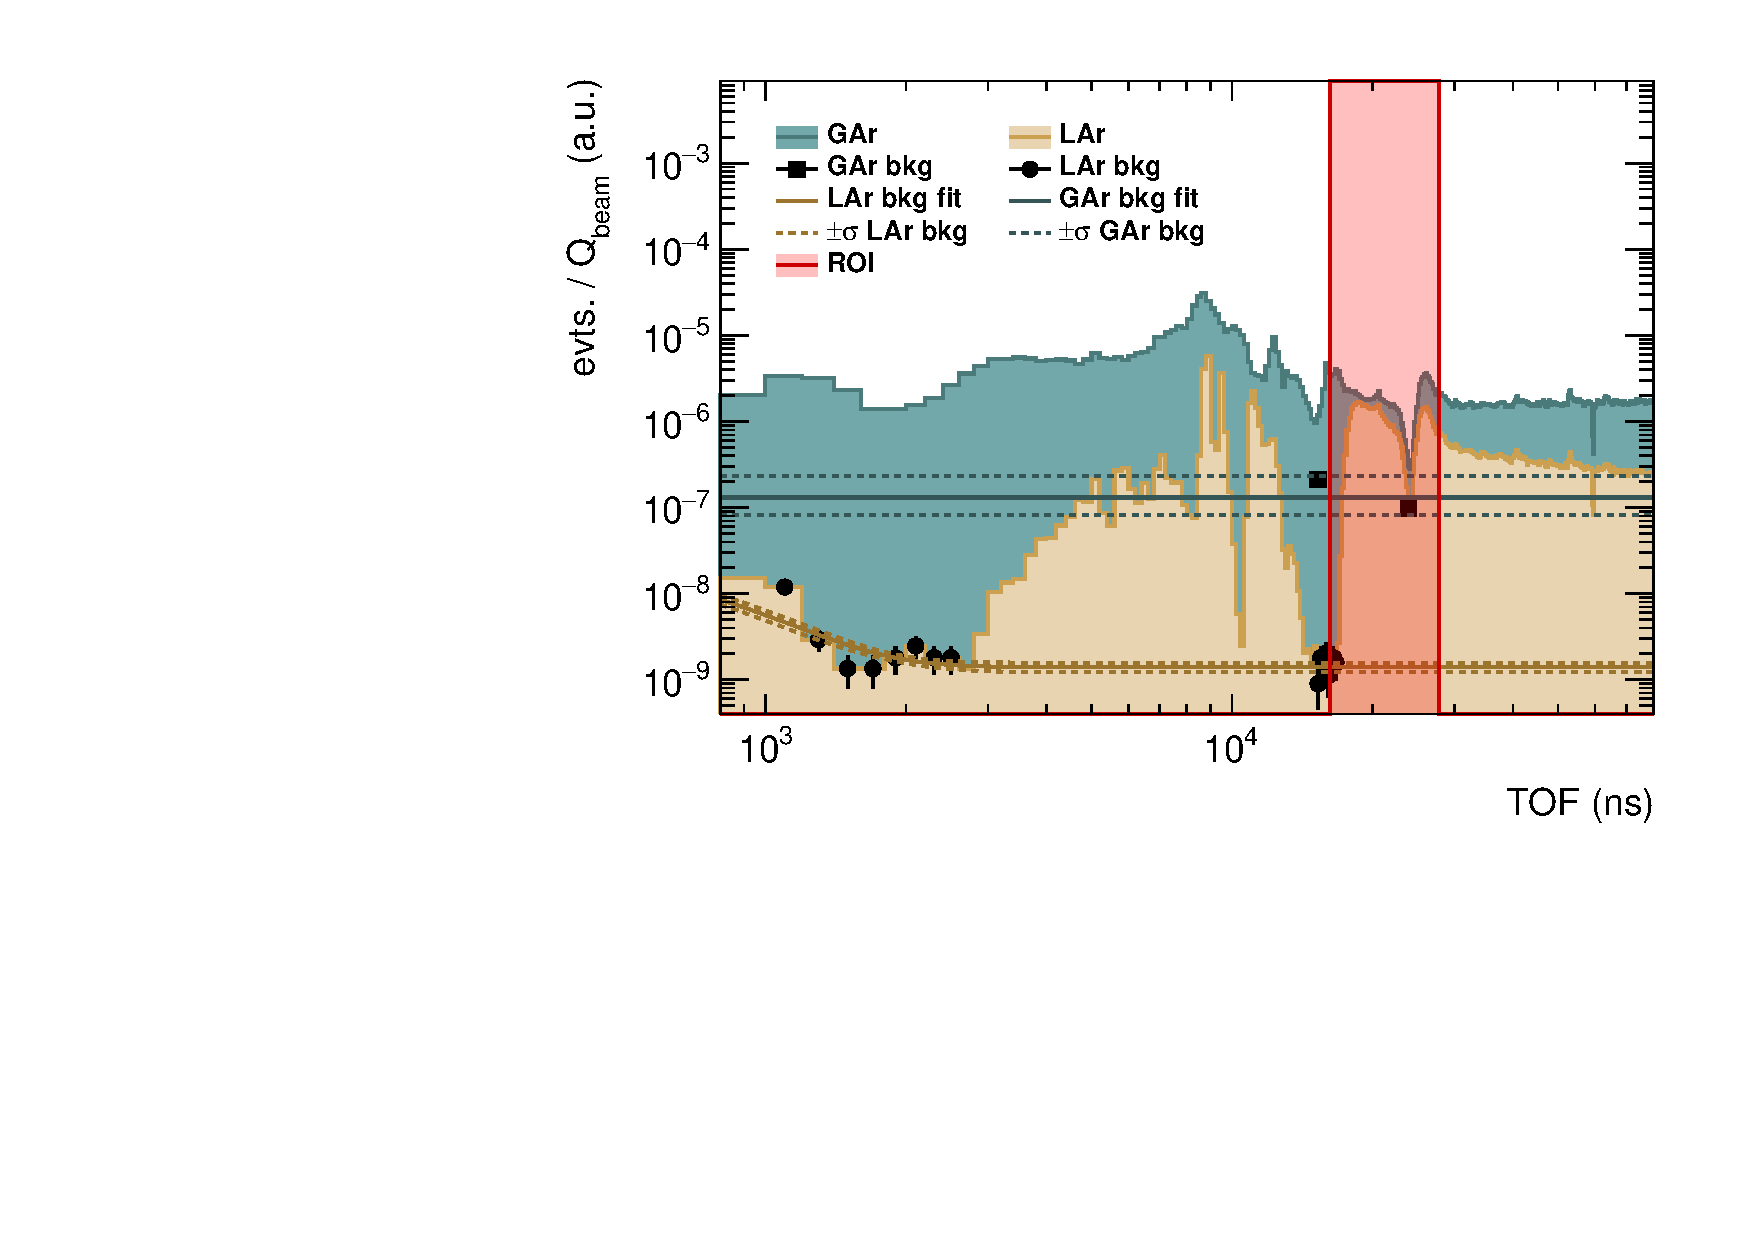
\includegraphics[width=\linewidth]{Figures/background.pdf}
\caption{Extraction of beam-related backgrounds.}
\label{fig:bkg}
\end{figure}

As shown in Fig.~\ref{fig:bkg}, the background analysis is done in
bins of TOF where the background is quite flat.  The background
differs for liquid and gas fills, as the neutrons reaching the
detector at the end of the beam line differ by more than an order of
magnitude.  The statistically significant background estimates from
Equation~\ref{eq:B} are fit to an exponential and constant for liquid
argon, and to a constant for gaseous argon.  The exponential feature
has neglible effect in the ROI.  Overall the background contribution
is {\color{red} $X\%$} for liquid argon and $2.64\%$ for gaseous
argon.

\section{Calibration}

The neutron detector records a time-of-flight (TOF) which, when
calibrated, determines the kinetic energy of each neutron event.
Each neutron scatters inside the moderator for an unknown time.  The
average time spent in the moderator $t_{\rm mod}$ can be determined
from the energy-dependent probability distribution, or moderator
function, which has has been determined for the LANSCE facility by
Monte Carlo simulation\cite{moderator}.  The velocity $v$ of each
neutron, and thus the kinetic energy $E$, is calculated from the
measured TOF $t$ as:
\begin{equation}
  v(t) = \frac{L_{\rm fit}}{ t - t_{\rm mod}(t) + t_{\rm fit} } 
\label{eq:v(t)}
\end{equation}
where $L_{\rm fit}$ and $t_{\rm fit}$ are parameters determined by
fitting features in the collected TOF data to known resonances of
aluminum and cadmium, both present in the beamline, and argon.  The
TOF-dependent moderator correction $t_{\rm mod}(t)$ is determined from
the energy dependent correction using an iterative
procedure.

In our energy ROI, the TOF for neutrons traversing the flight path
varies by $9~{\rm \mu s}$, and the moderator correction is typically
$1-2\%$.  The best fit value of $L_{\rm fit}$ is $63.82~\rm m$ which
agrees well with physical measurements made along the beam line.  The
parameter $t_{\rm fit}$ accounts for time delays in the Li-glas
detector, cables, and the DAQ system, as well as any residual
difference between the actual and simulated moderator response.

The energy resolution is primary limited by the width of the moderator
function $\sigma(t_{\rm mod}$ which is typically $10\%$ of the TOF.
The incident neutron pulse, which has a triangular shaped pulse with
FWHM of 125 ns, contains $68\%$ within $\sigma(t_0) = 53~\rm ns$.

\begin{table}[h!]
    \centering
    \begin{tabular}{|c|c|c|c|c|}
    \hline
    E & TOF &  $\sigma(t_{0})$ & $\pm \sigma(t_{\rm mod})$  & $\pm \Delta E/E$ \\
    (keV) & (ns) & (ns) & (ns) & ($\%$) \\\hline 
    30-40 & 24816 & 53 & +334, -130 & +2.7, -1.0\\
    40-50 & 21861 & 53 & +341, -146 & +3.1, -1.3\\
    50-60 & 19744 & 53 & +313, -128  & +3.1, -1.3\\
    60-70 & 18134 & 53 & +286, -120  & +3.1, -1.3\\\hline
    \end{tabular}
    \caption{Main sources of uncertainties in TOF contributing to the energy resolution. {\color{red} minor updated from Jingbo needed since removal of $t_d$.}}
    \label{tab:tof_error}
\end{table}

The use of gaseous argon fill during target out runs, instead of
vacuum, is accounted for in the effective target number density:
\begin{equation}
  n_{\rm trg} = n_{\rm in} - n_{\rm out}
\label{eq:rho(E)}
\end{equation}
where $n_{\rm in}$ is the argon number density for liquid argon fills
and $n_{\rm out}$ is for gaseous argon fills.  {\color{red} [Temperature and pressure of gaseous argon used?]}

The ARTIE vessel was held at atmospheric pressure, so the argon was
continuously boiling during liquid fills.  The number density $n_{\rm
  in}$ of the boiling liquid argon was measured directly in a separate
experiment at UC Davis.  The entire target assembly was placed on a
precision scale, one of the argon dewars was instrumented with a
stainless-steel ruler, and a video camera was arranged to
simultaneously record the scale and ruler.

The scale was calibrated to detector volume by incrementally filling
the vessel with known volumes of water, and the mass of the target
apparatus was determined when the vessel was filled with air.  The
target was filled with liquid argon, and recorded during the boil off
period.  To avoid measurement instability resulting from large bubbles
emerging from the dewar, our analysis excludes volume readings which
were not stable to within $25~\rm mL$ for a 1 second time interval.
The detector volume as function of time was linear with a measured
boil-off rate of $1.56~\rm L/hr$, consistent with our filling rate of
$1.5$ to $2.0~\rm L/hr$ while conducting the experiment.  The
effective target density was determined to be $n_{\rm in} = 1.318 \pm
0.017~{\rm kg/L}$.  The analysis included corrections for the thermal
expansion of the target vessel, the additional weight from ice forming
on the window, and the difference in altitute between UC Davis and Los
Alamos.  [How was uncertainty determined?]

Despite being flushed continuosly with dry nitrogen gas, the kapton
{\color{red} [text originally said mylar?]} windows located at each
end of the target developed a thin layer of ice during liquid argon
runs.  Once the ice buildup reached $\sim 5~\rm mm$, the target was
warmed up to melt the ice.  The transmission coefficient for the ice
at its maximum thickness was determined from Eq.~\ref{eq:T} with runs
taken immediately before each warm-up, with maximal ice build-up, used
as ``target in'', and runs taken immediately after the warm-up, with
minimal ice build-up, used as ``target out''.  A Monte Carlo
simulation was used to determine the transmission coefficient of ice
using the incident neutron spectrum and the ENDF total cross-section.
The best-fit ice thickness was found to be $d =
0.030^{+0.095}_{-0.025}~\rm cm$, which is consistent with our
observation that $5~\rm mm$ ice powder consisted of ice crystals mixed
with a significant amount of air.

\section{\label{sec:energy}Systematic Uncertainties}

\begin{table}[h!]
    \centering
    \begin{tabular}{|c|c|c|c|}
\hline
& affected & parameter & cross-section  \\
    name & parameters & uncertainty & uncertainty \\ \hline        
beam instability & $Q_{\rm in}, Q_{\rm out}$ & $\pm 1.0\%$ & $\pm$1.0\%\\   
thermal misalignment & $Q_{\rm in}$ & -5\% & -3.1\% \\
boiling & $n_{\rm in}$ & $\pm$1.3\% & $\pm$1.3\%\\
ice buildup & $Q_{\rm in}$ & $-$3.8\% & $-$2.4\%\\   
atmospheric pressure & $n_{\rm eff}$ & $\pm 0.4\%$ & $\pm 0.4\%$ \\
target-in background & $B_{\rm in}$ & & \\
target-out background & $B_{\rm out}$ & & \\
\hline
    \end{tabular}
    \caption{Summary of systematic uncertainties. {\color{red} updated needed from Mike}}
    \label{tab:uncertainties}
\end{table}

The stability of the beam, beam monitoring, target alignment, and
neutron detector efficiency was assessed during special runs during
which the target vessel contained air.  An analysis of the average
neutron rate during two days of running at the start the experiment
and one day of running at the end showed that these systematic effects
remained within $1.1\%$.

The event selection removes the time period immediately following each
liquid argon fill during which the observed neutron rate was less than
$95\%$ of the plateau rate.  We assess a one-sided $-5\%$ systematic
uncertainty which we attribute to transient inadvertent thermal
misalignment of the collimators after each fill.

The number density of boiling liquid argon in the target was
experimentally determined with an associated systematic uncertainty of
$1.3\%$.  {\color{red} [I took this from 0.17/1.318.. differs from value in the table of 1.5\%  How was this uncertainty determined?]}

The measured cross-section was not corrected for ice buildup on the
kapton windows.  Instead, the simulated transmission coefficient for
ice with a thickness equal to the $1~\rm sigma$ upper bound on
experimentally determined maximum ice thickness ($1.3 \rm cm$) is
taken as a one-sided systematic uncertainty ($-3.8\%$) on the beam
intensity.
  
The last $2~\rm m$ of the flight path is housed in a non-temperature
controlled building.  During the course of the data taking, the
average air density was found to be $0.85~{\rm mg/cm^3}$ with a maximum of
$0.95 \ mg/cm^3$ and a minimum of $0.75~{\rm mg/cm^3}$, using data
collected from the TA-53 (LANSCE) and TA-54 (White Rock) weather
stations.  The maximum variation in the neutron flux reaching the
detector was calculated from the maximum variation in the air density
and the known cross-section for the three main constituents of air.
The variation $0.4\%$ was applied as a systematic due to atmospheric
pressure.

After our selection cuts, several systematic uncertainties were
determined to be neglible, including those from: non-linearity between
the beam intensity and CT measurement, dead time in the data
acquisition system, PMT afterpulsing, and contamination of the argon
gas.

The absolute energy calibration is limited by the statistical
uncertainties on the fitted parameter $\sigma(t_{\rm fit})=29~\rm ns$,
and the contribution from $\sigma(L_{\rm fit})=0.064~\rm m$ is
neglible.  No systematic uncertainty for energy resolution is applied
to the cross-section results, which are reported as function of
measured energy.


\section{\label{sec:energy}Conclusions}

From the experimentally determined neutron counts in each TOF bin, the
transmission coefficient $T$ is calculated from Eq.~\ref{eq:T} and the
cross-section from Eq.~\ref{eq:sigma}.  The central value of each TOF
bin is coverted to energy using Eq~\ref{eq:v(t)}, which determines the
kinetic energy dependence of these experimentally determined
quantities.

\begin{figure}[htbp]\centering
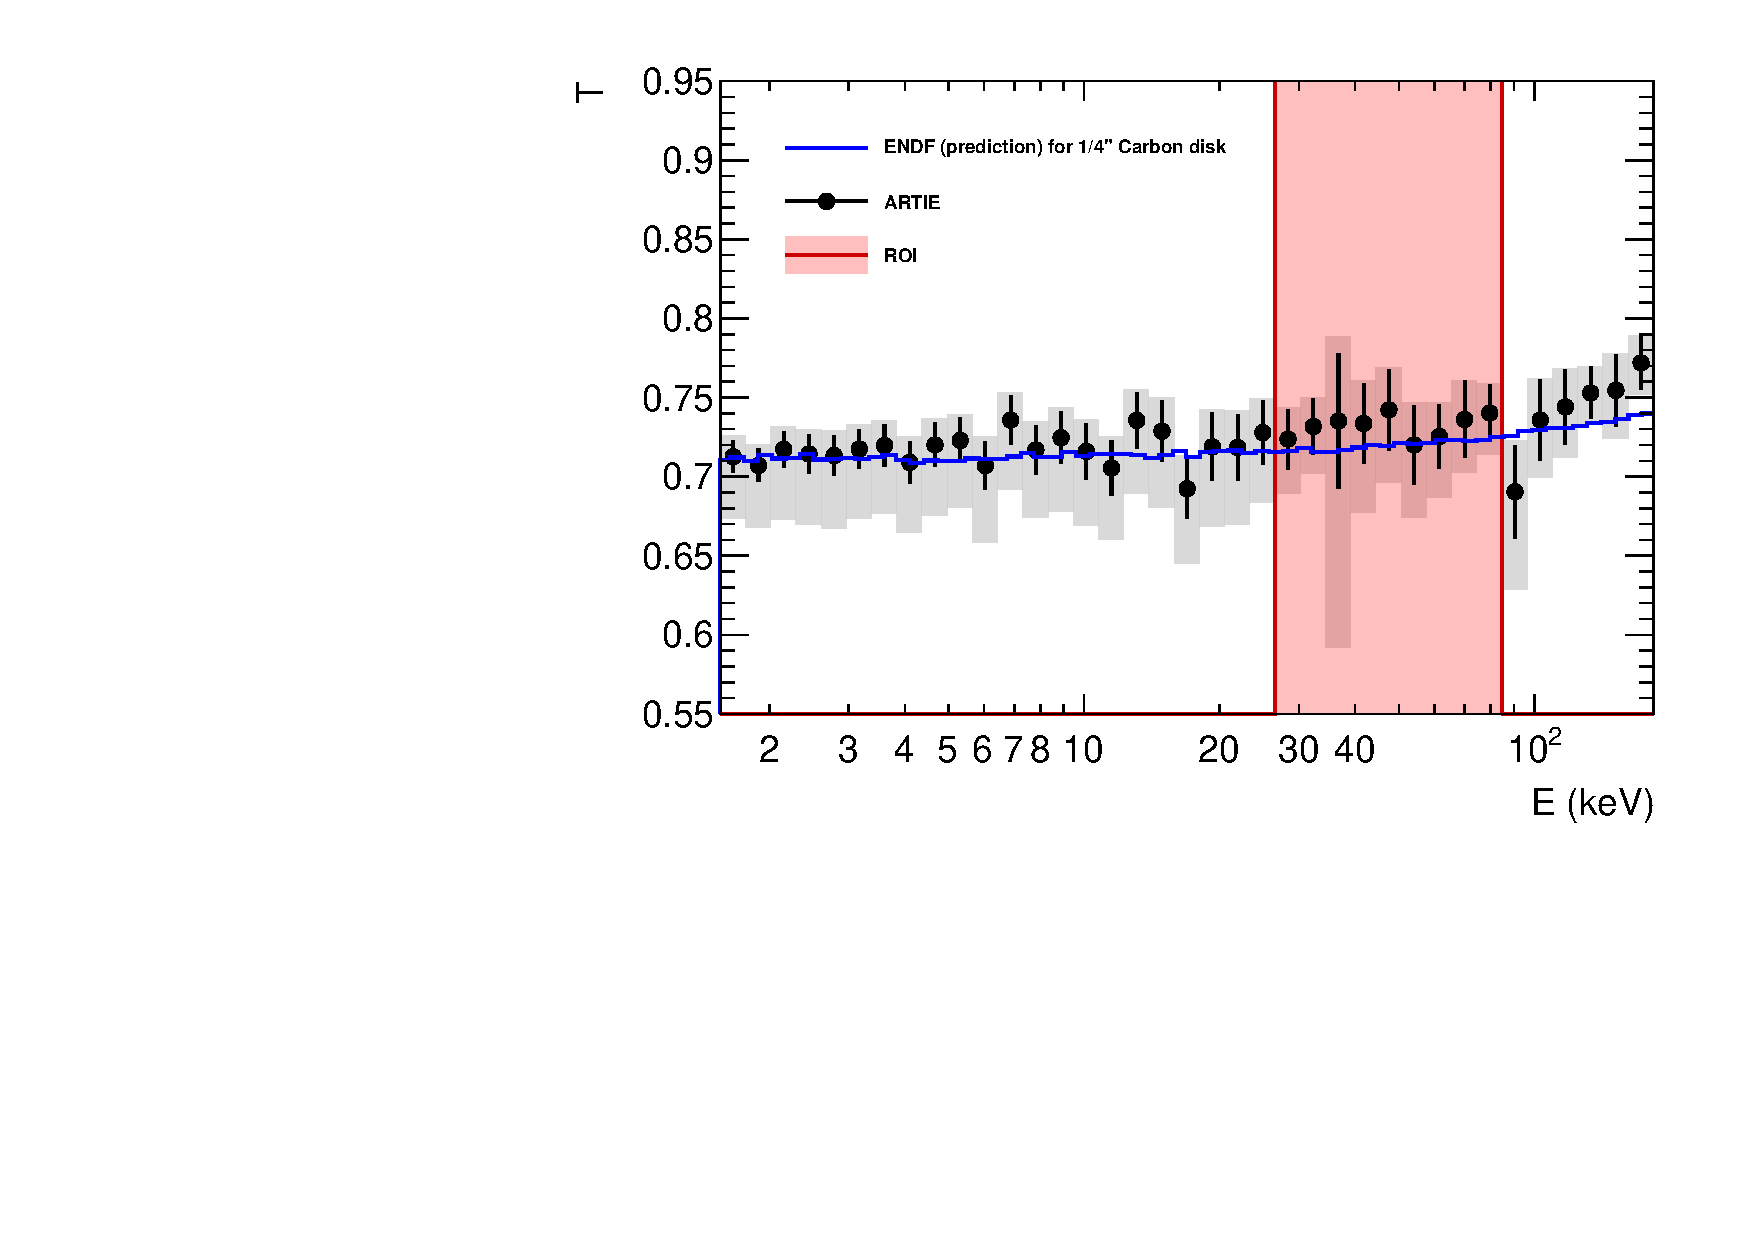
\includegraphics[width=\linewidth]{Figures/carbon.pdf}
\caption{Transmission coefficient $T$ obtained for two $0.125\pm 0.010$” thick carbon (99.999\% purity) disk inserted in the beam line attached to the ARTIE target. Good agreement ($\chi^{2}/\text{NDF} = 2.7 / 6 = 0.45$ in the ROI) is found with the theoretical prediction of $T$ obtained using the carbon cross section tabulated in ENDF and smeared by the measured energy resolution of ARTIE.}
\label{fig:carbon}
\end{figure}

As a cross check of the experimental methods and analysis procedure,
the cross-section of carbon was determined from data collected with
two $0.125\pm 0.010$” thick carbon (99.999\% purity)
disks~\cite{CarbonLesker} attached to the ARTIE target while it was
flushed with gaseous argon.  Fig.~\ref{fig:carbon} shows the
measured transmission coefficient $T(E)$ as a function of the energy
compared to the theoretical prediction from ENDF smeared by the
detector energy resolution.  Good agreement
($\chi^{2}/\text{NDF} = 2.7 / 6 = 0.45$
in the ROI) was found.

\begin{figure}[h!]
    \centering
    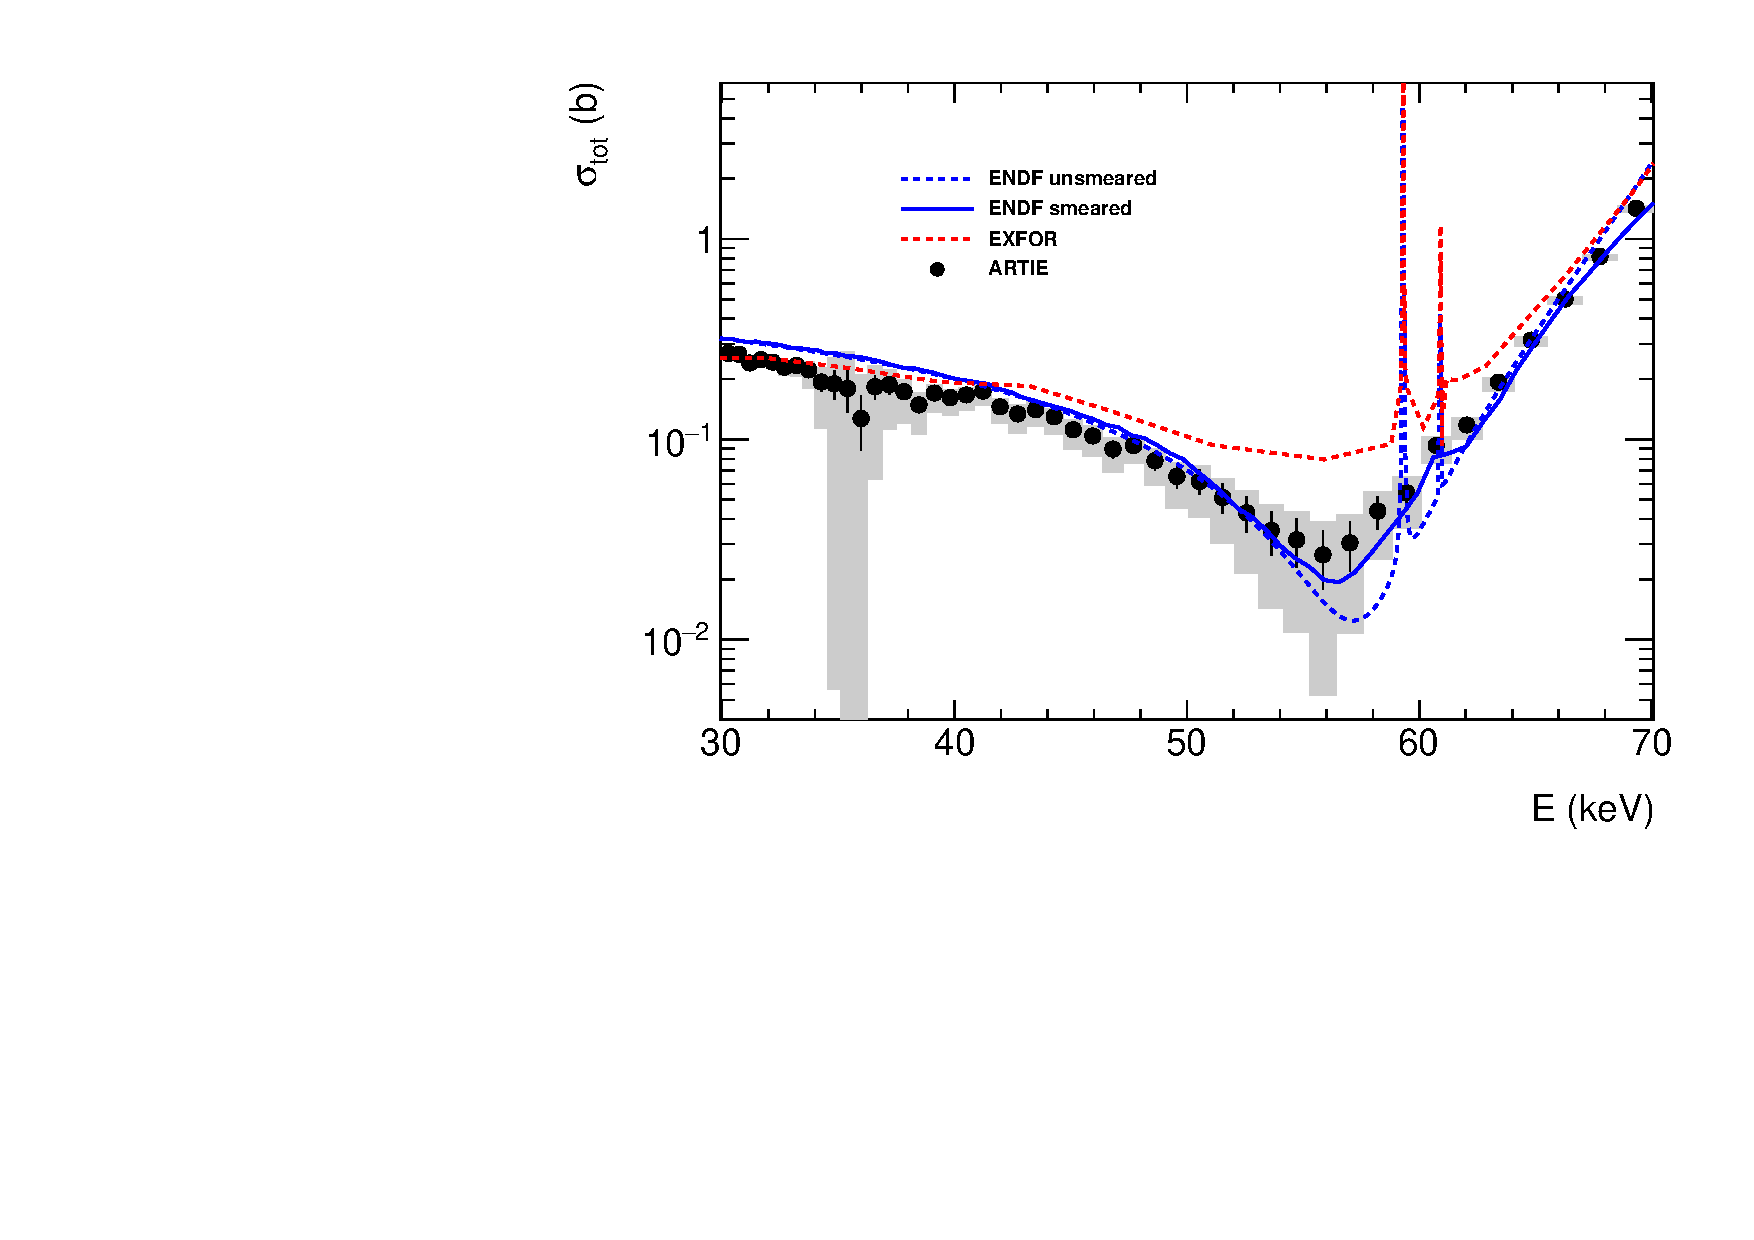
\includegraphics[width=\linewidth]{Figures/cross-section.pdf}
    \caption{Neutron-argon total cross section as a function of energy}
    \label{fig:results}
\end{figure}

The measured neutron-argon total cross-section as a function of
kinetic energy is shown in Fig.~\ref{fig:results}.  Our results are
consistent with the prediction from the ENDF cross-section smeared by
the ARTIE energy resolution for the range from $40$ to $70~\rm keV$.
In the region from $30$ to $40~\rm keV$ our results reproduce the
EXFOR results which differ from the ENDF prediction.
{\color{red} [In addition, at 35 keV aluminum also has a large
    resonance (34 barns) that limits statistics, as the vacuum beam
    pipe flanges are made of aluminum.]}
The EXFOR experiment was optimized for a scan of a
much wider energy region and higher cross-section, and our results
only differ for cross-sections less than $0.2~\rm b$.  We suspect that
our results are consistent if statistical uncertainty of the EXFOR
results in the regions of low cross-section are accounted for.  Our
results confirm the predicted anti-resonance feature at $57~\keV$,
which has profound implications on the ability of neutrons to traverse
large distances in liquid argon detectors and shielding.


\section{\label{sec:acknowledgments}ACKNOWLEDGEMENTS}

This work was supported by the U.S. Department of Energy (DOE) Office
of Science under award number DE-SC0009999, and by the DOE National
Nuclear Security Administration through the Nuclear Science and
Security Consortium under award number DE-NA0003180. This work was
supported by the U.S. Department of Energy through the Los Alamos
National Laboratory. Los Alamos National Laboratory is operated by
Triad National Security, LLC, for the National Nuclear Security
Administration of U.S. Department of Energy (Contract
No. 89233218CNA000001).  We gratefully acknowledge the logistical and
technical support and the access to laboratory infrastructure provided
to us by LANSCE and its personnel.


\section{Bibliography}

\bibliographystyle{unsrt}
\bibliography{bibliography.bib}

\end{document}

\subsection{Measurement Strategy}
\label{sec:strategy}

The ARTIE experiment determines the neutron total cross-section in argon using the one-dimensional geometry illustrated.

The kinetic energy (E) of each detected neutron can be determined from the Time-Of-Flight (TOF) $t$ by the relativistic formula:
\begin{equation} \label{eq:tof}
E = m c^2 \left[\frac{1}{\sqrt{1-L^2/c^2t^2}}-1 \right]
\end{equation}
where $m$ is the mass of the neutron, $L$ is the flight distance, and $t$ is the flight time.  In practice, the actual distance traversed by the neutron is greater than $L$ because the path of each neutron through the neutron moderator needs to be considered.  The average extra distance in the moderator is known as the {\it Moderator Response Function} (MRF) and is determined by simulation and validated by data from known neutron cross-section resonances, as discussed in Sec.~\ref{sec:ecal}.
%%Sofia, need to introduce also L (and T0?). The moment and position of the neutron production is given by the beam instrumentation. $L$ is set to be the distance between the (...) and detector. In practice, the actual distance (...). A simulation of the effect of the moderator is used to provide an average correction and the energy resolution, at each energy measured with eq. 1.

The ARTIE target was designed such that the target volume may contain liquid argon (LAr), gaseous argon (GAr), or air. For any given target fill, the number of neutrons of energy $E$ which reach the TOF detector during a particular run is given by:
\begin{equation}
N(E) = f(E) Q T(E)
\end{equation}
where $Q$ is the total number of neutrons produced during the run and $f(E)$ is a source term that depends on neutron beam energy profile, the amount and type of material present in the beam line and target assembly, the beam line acceptance, and the neutron detector efficiency. $T(E)$ is the probability that a neutron can traverse the material in the target without interaction. This is commonly referred to as the {\it transmission coefficient}.

If the target is filled with argon of density $n$ atoms/$cm^3$, the probability $T$ that a neutron will not scatter while traversing a distance $d$ is then given by:
\begin{equation}
T(E) = e^{-n d\sigma}
\label{eq:P(E)}
\end{equation}
where $\sigma$ is the total neutron-argon cross-section we seek to measure.  
%Because neutrons do not experience ionizing energy loss while traversing the target, the energy is constant, and the probability that a neutron traverses the entire target length ($d$) without scattering is determined by integration:
The quantity $n d$ is called the target thickness and has units of atoms per barn.  The total number of neutrons that reach the 6-Li detector without interacting is given by:
\begin{equation}
N(E) = f(E) Q e^{-n d \sigma}
\end{equation}
%Since we are only considering neutrons that do not scatter, and neutrons do not experience continuous ionization energy loss, the factor $f(E)$ is the same factor for all target fill materials.
%%Sofia: neutrons that reach the TOF? Maybe: neutrons of energy E that reach the detector n(E) is experimentally determined from TOF.
To avoid the need to determine the absolute value of the factor $f(E)$ the following procedure is used:

The total neutron-argon cross-section $\sigma(E)$ is determined from data collected with the target in two different configurations.  For ``target-in'' runs the volume contains LAr, a total number of neutrons $Q_{\rm liq}$ is produced, and the number of neutrons of energy $E$ that reach the detector $N_{\rm liq}(E)$ is experimentally determined.  For ``target-out'' runs, the target volume would ideally be at vacuum, but in practice GAr is used. The total number of neutrons produced is given by $Q_{\rm gas}$, and the number of neutrons detected is given as $N_{\rm gas}(E)$.

The factor $f(E)$ is assumed constant to within the systematic uncertainties as discussed below. Thus, the total cross-section can be calculated as:
\begin{equation}
\sigma(E) = -\frac{1}{(n_{\rm liq}-n_{\rm gas}) d} \, \ln \left( \frac{N_{\rm liq}(E)/Q_{\rm liq}}{N_{\rm gas}(E)/Q_{\rm gas}} \right) \\
\label{eq:sigma}
\end{equation}
Because the quantity $Q$ is only used as a ratio, any quantity proportional to the number of neutrons produced can be used.  The ARTIE experiment uses the integrated proton beam current as measured by a beam Current Transformer (CT). Systematic uncertainties associated with the CT are discussed in Sec.~\ref{sec:beamstability}.

The single-interaction analysis described here does not account for processes involving scatters outside of the target and beam line which reach the 6-Li detector.  This background is measured (Sec.~\ref{sec:backgrounds}) and subtracted from the experimentally determined counts.
t.


